\section{Greenplum Database}
\label{sec:greenplum}

\href{http://greenplum.org/}{Greenplum Database (GP)}~--- реляционная СУБД, имеющая массово-параллельную (massive parallel processing) архитектуру без разделения ресурсов (shared nothing). Для подробного понимания принципов работы Greenplum необходимо обозначить основные термины:

\begin{itemize}
  \item Master instance (<<мастер>>)~--- инстанс PostgreSQL, являющийся одновременно координатором и входной точкой для пользователей в кластере;
  \item Master host (<<сервер-мастер>>)~--- сервер, на котором работает master instance;
  \item Secondary master instance~--- инстанс PostgreSQL, являющийся резервным мастером, включается в работу в случае недоступности основного мастера (переключение происходит вручную);
  \item Primary segment instance (<<сегмент>>)~--- инстанс PostgreSQL, являющийся одним из сегментов. Именно сегменты непосредственно хранят данные, выполняют с ними операции и отдают результаты мастеру (в общем случае). По сути сегмент~--- самый обычный инстанс PostgreSQL 8.2.15 с настроенной WAL-репликацией в своё зеркало на другом сервере;
  \item Mirror segment instance (<<зеркало>>)~--- инстанс PostgreSQL, являющийся зеркалом одного из primary сегментов, автоматически принимает на себя роль primary в случае падения оного. Greenplum поддерживает только 1-to-1 репликацию сегментов: для каждого из primary может быть только одно зеркало;
  \item Segment host (<<сервер-сегмент>>)~--- сервер, на котором работает один или несколько сегментов и/или зеркал;
\end{itemize}

В общем случае кластер GP состоит из нескольких серверов-сегментов, одного сервера-мастера, и одного сервера-секондари-мастера, соединённых между собой одной или несколькими быстрыми (10g, infiniband) сетями, обычно обособленными (interconnect) (рис~\ref{fig:greenplum1}).

\begin{figure}[h!]
  \center{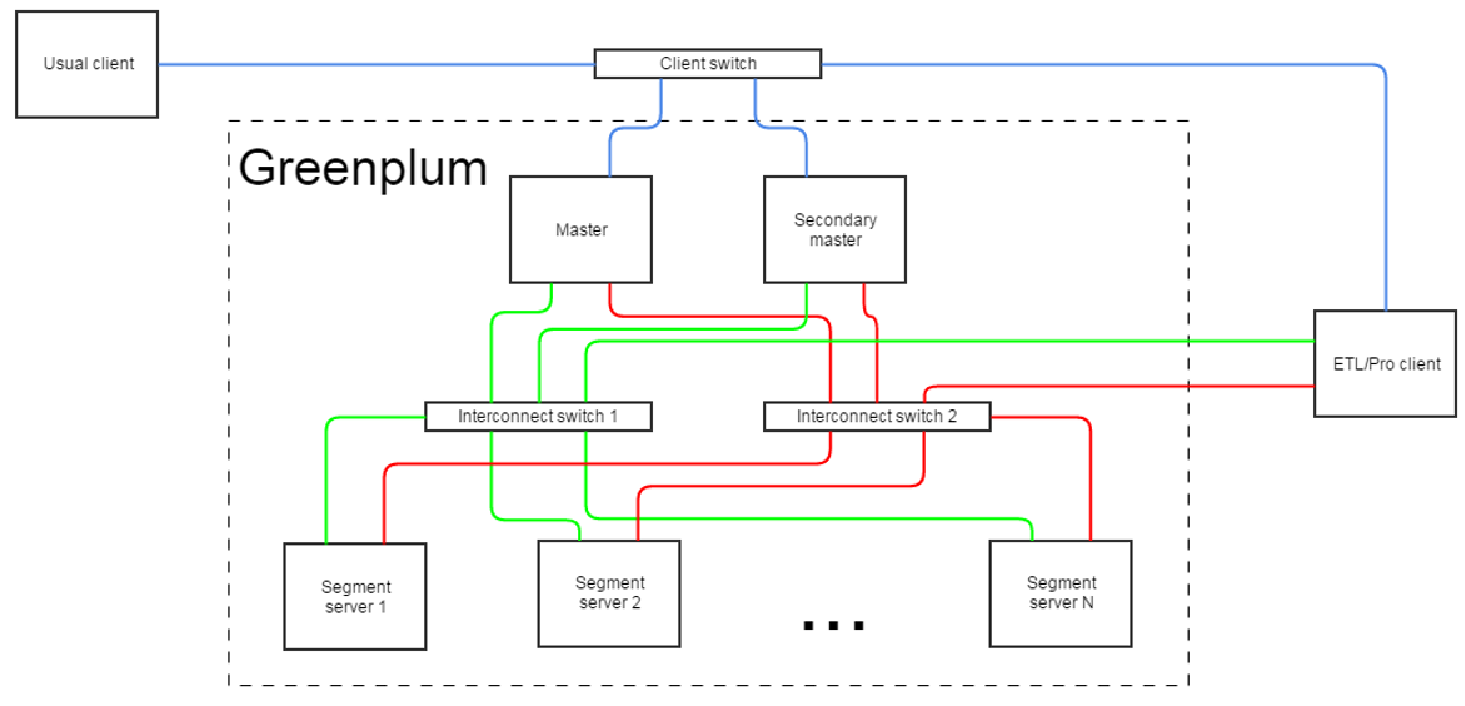
\includegraphics[width=1\textwidth]{greenplum-basic-arch.pdf}}
  \caption{Состав кластера и сетевое взаимодействие элементов. Зелёная и красная линии~--- обособленные сети interconnect, синяя линия~--- внешняя, клиентская сеть}
  \label{fig:greenplum1}
\end{figure}

Использование нескольких interconnect-сетей позволяет, во-первых, повысить пропускную способность канала взаимодействия сегментов между собой, и во-вторых, обеспечить отказоустойчивость кластера (в случае отказа одной из сетей весь трафик перераспределяется между оставшимися).

При выборе числа серверов-сегментов важно правильно выбрать соотношение кластера <<число процессоров/Тб данных>> в зависимости от планируемого профиля нагрузки на БД~--- чем больше процессорных ядер приходится на единицу данных, тем быстрее кластер будет выполнять <<тяжёлые>> операции, а также работать со сжатыми таблицами.

При выборе числа сегментов в кластере (которое в общем случае к числу серверов никак не привязано) необходимо помнить следующее:

\begin{itemize}
  \item все ресурсы сервера делятся между всеми сегментами на сервере (нагрузкой зеркал, в случае если они располагаются на этих же серверах, можно условно пренебречь);
  \item каждый запрос на одном сегменте не может потреблять процессорных ресурсов больше, чем одно ядро CPU. Это означает, например, что, если кластер состоит из 32-ядерных серверов с 4-я сегментами GP на борту и используется в среднем для обработки 3-4 одновременных тяжёлых, хорошо утилизирующих CPU, запросов, <<в среднем по больнице>> CPU не будет утилизироваться оптимально. В данной ситуации лучше увеличить число сегментов на сервере до 6-8;
  \item штатный процесс бекапа и рестора данных <<из коробки>> работает только на кластерах, имеющих одинаковое число сегментов. Восстановить данные, забекапленные на кластере из 96 сегментов, в кластер из 100 сегментов без напильника будет невозможно;
\end{itemize}
